\documentclass{report}

\usepackage{graphicx}
\usepackage{hyperref}
\usepackage{tikz}
\usepackage{pgfplots}
\usepackage{multirow}
\usepackage{tabulary}


\author{Mihalache Radu-Stefan}
\date{}
\title{}


\begin{document}
\begin{center}
\Large
\textbf{Study of function minima using Hill Climbing, Simulated Annealing and Genetic algorithms}
        
\vspace{0.4cm}
\textbf{Mihalache Radu Stefan}
       
\vspace{1.2cm}
\textbf{Abstract}

\end{center}

\vspace{0.4cm}
In this paper I will approach the problem of solving the global minima with Hill Climbing,  Simulated Annealing and Genetic algorithms,
use my implementation to compare their performance and draw soime conclusions regarding their efficiensy.


\section*{Introduction}
\subsection*{Motivation}
The problem of exploring the values of functions and finding the global minimum of said function for a specified domain has useful aplications, yet it is dificult to solve with a deterministic algorithm.
That is because some functions have a very small accumulation basins compared with the size of the domain for the global minimum.

\begin{figure}[!h]
  \centering
\begin{tikzpicture}
  \begin{axis}[
      xlabel=x,
      ylabel=$f(x)$
    ]
    \addplot [
      color=red,
      mark=x
    ]
    coordinates {
      (0, 5)
      (1, 5.1)
      (2, 5.2)
      (3, 5.3)
      (3.3, 0)
      (3.5, 5.4)
      (7, 5.5)
    };
  \end{axis}
\end{tikzpicture}
\end{figure}
\pagebreak

To solve this problem we will explore the following nondeterministic approaches:
\newline
\hspace*{10mm} - The Hill Climbing algorithm which is a greedy methode
\newline
\hspace*{10mm} - The Simulated Annealing algorithm which is a meta-heuristic methode that better explores the function's domain
\newline
\hspace*{10mm} - The Genetic algorithm which takes inspiration from nature and addapts its solution population to get closer to the global minimum
\newline
\newline
The motivation of this experiment is to dertermine which one of the approaches listed above gives 
the best results for a set of functions  in the shortest ammount of time and examine why. 

\section*{Method}

The representation of the input variables will be a string of n bits such that they can accuately represent the function domain.

$$x = a + decimal_{represenation}(bit_{str}) \cdot (b - a)/(2^n - 1) ,  x \in \left[a, b \right]$$

Hill Climbing and Simulated annealing make use of this represenattion by generating a random input called the candidate solution, its vecinity can be explored by negating one bit, such that the hamming distance between the candidate solution and the vecinity is one.
\newline
\newline
\textbf{Hill Climbing}:
\newline
\newline
Selects a candidate solution for each iteration and try to improove it using either the first better vecinity (first improovement) or the best vecinity (best improovement). 
This algorithm finds the minimumm by exploring the basin of the candidate solution.
\newline
\newline
\textbf{Simulated annealing}:
\newline
\newline
Selects a candidate solution at the start and explore its vecinity. This algorithm better explores the domain of the function by choosing worse vecinities base on the probability given by this expression:
\newline
$$random.uniform(0, 1) < math.exp(-abs((evaln - evalc) / temperature))$$
\newline
This algorithm makes use of the hot iron concept. At the begining the temperature  is high and the chance to choose a worse solution is high but it decreeses over each iteration 
(which makes it more greedy)  based on this formula:
\newline
$$temperature = temperature \cdot 0.9$$

\pagebreak

\noindent
\textbf{Genetic}:
\newline
\newline
The genetic algorithm takes inspiration from nature, by holding a population of chromosomes which are selected and evolve under the pressure a a fitness function.
A chromosome represents a potential solution and its chanses to be selected for the next generation depend on the chromosome's evaluation by the fitness function.
As the solution is set of bits, a gene is an individual bit in the solution. The evolution process is acomplished by performing mutation and cross over on the chromosomes of the population.
\newline
\newline
Mutation is performed by fliping a random bit of a chromosome.
\newline
\newline
Crossover at one point between two chromosomes is performed by piking a random locus (position of a gene) and swaping the genes after thge locus between the two. Example, locus = 4 :
$$10101010 \rightarrow 10101111 $$
$$11111111 \rightarrow 11111010 $$
\newline
The fitness function $fit(chromosome)$ that I have used in this experiment is inversely proportional with the result of the function $f(chromosome)$ for which we want to find the minima.
It uses $maximum = max(f(current_{population}))$ and $minimum = min(f(current_{population}))$ .
\newline
$$fit(chromosome) = (maximum - f(chromosome)) / (maximum- minimum)$$
\newline
The selection mechanism I have used in this experiment is Wheel of Fortune. It calculates the totalFitness
$$totalFitness = \sum(fit(chromosome))  , chromosome \in population$$
in order to computes the individual probability $p_{chromosome} = fit(chromosome) /  totalFitness$
and an array of cumulated probabilities $q_{i + 1} = q_{i} + p_{chromosome_i}$ that it uses to a chromosome at position $j$,  $population_{size}$ times such that:
$$r \in \left(0, 1 \right] \, , \, q_j < r < q_{j + 1}$$
\newline
An additional mechanism my genetic algorithm implementation make use of is Elitism. It makes sure that the best x solutions are always maintained in the population and mitigates the effects
of evolutions that do not result in better solutiuons.

\pagebreak

\section*{The analysed functions:}

\begin{figure}[!h]
  \centering
  $$ f(x) = \sum_{i=1}^n \left[ x_i^2 \right],
   x_i \in \left[ -5.12, 5.15 \right]$$
   $$min = 0$$

  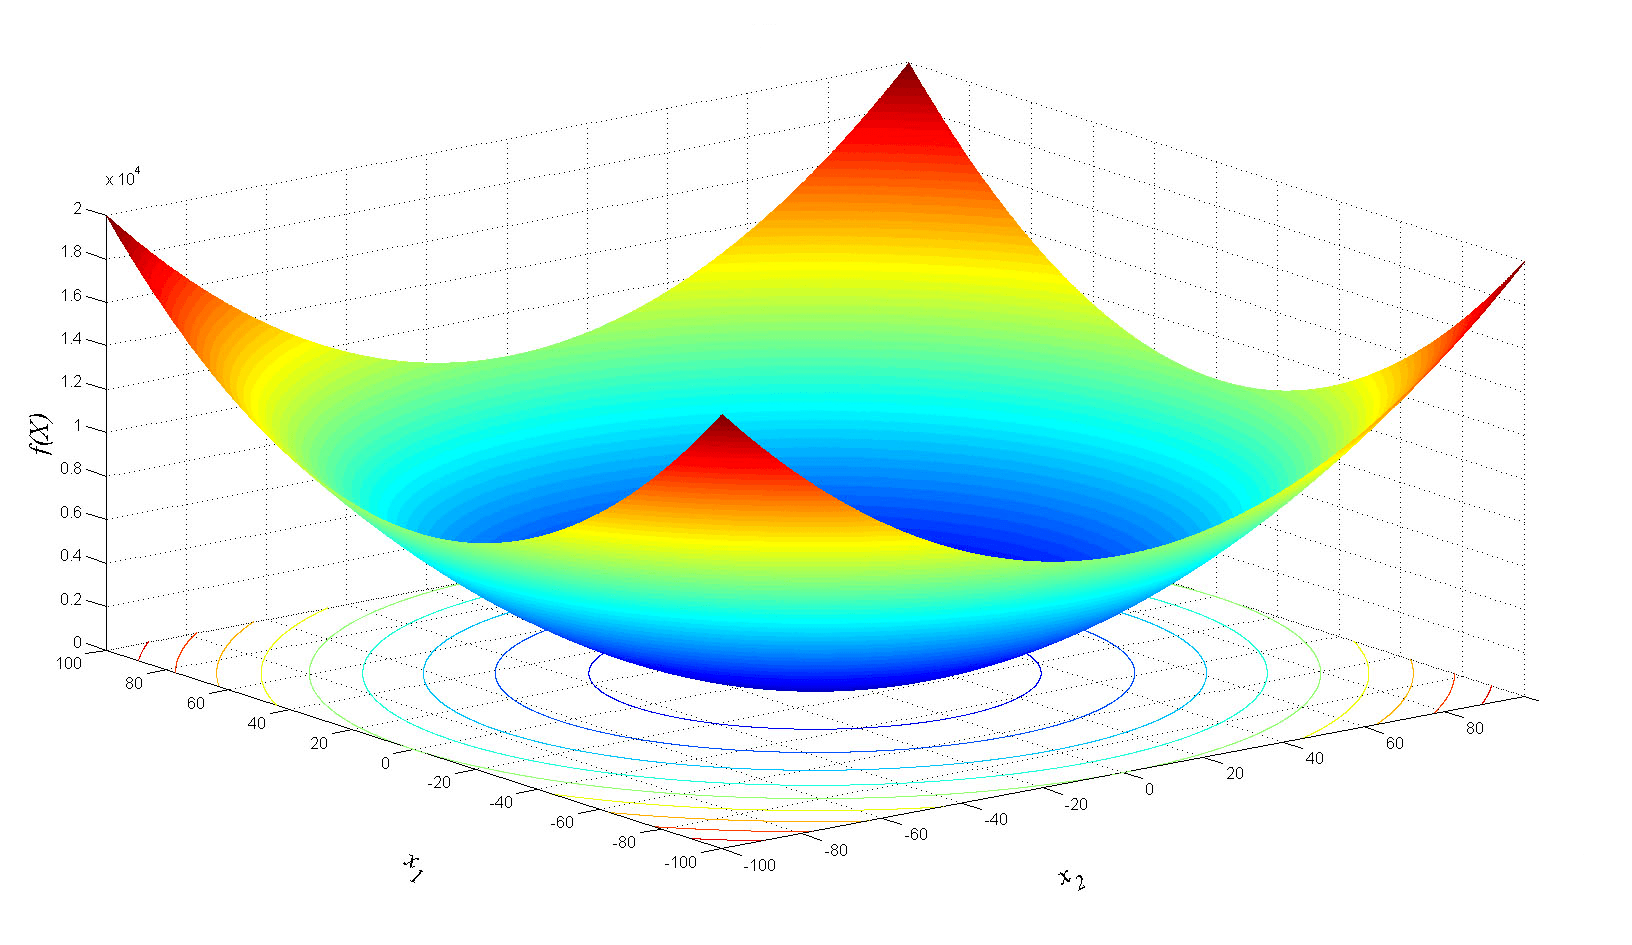
\includegraphics[width=100mm,scale=0.5]{De_Jong_function}
  \caption{Image De Jong's Function.\protect\footnotemark}
\end{figure}
\footnotetext{https://al-roomi.org/benchmarks/unconstrained/n-dimensions/}

\pagebreak

\begin{figure}[!h]
  \centering
  $$ f(x) = \sum_{i=1}^n \left[-x_i \cdot sin(sqrt(|x_i|)) \right],
   x_i \in \left[ -500, 500 \right]$$
   $$min = (-n) * 418.98$$

  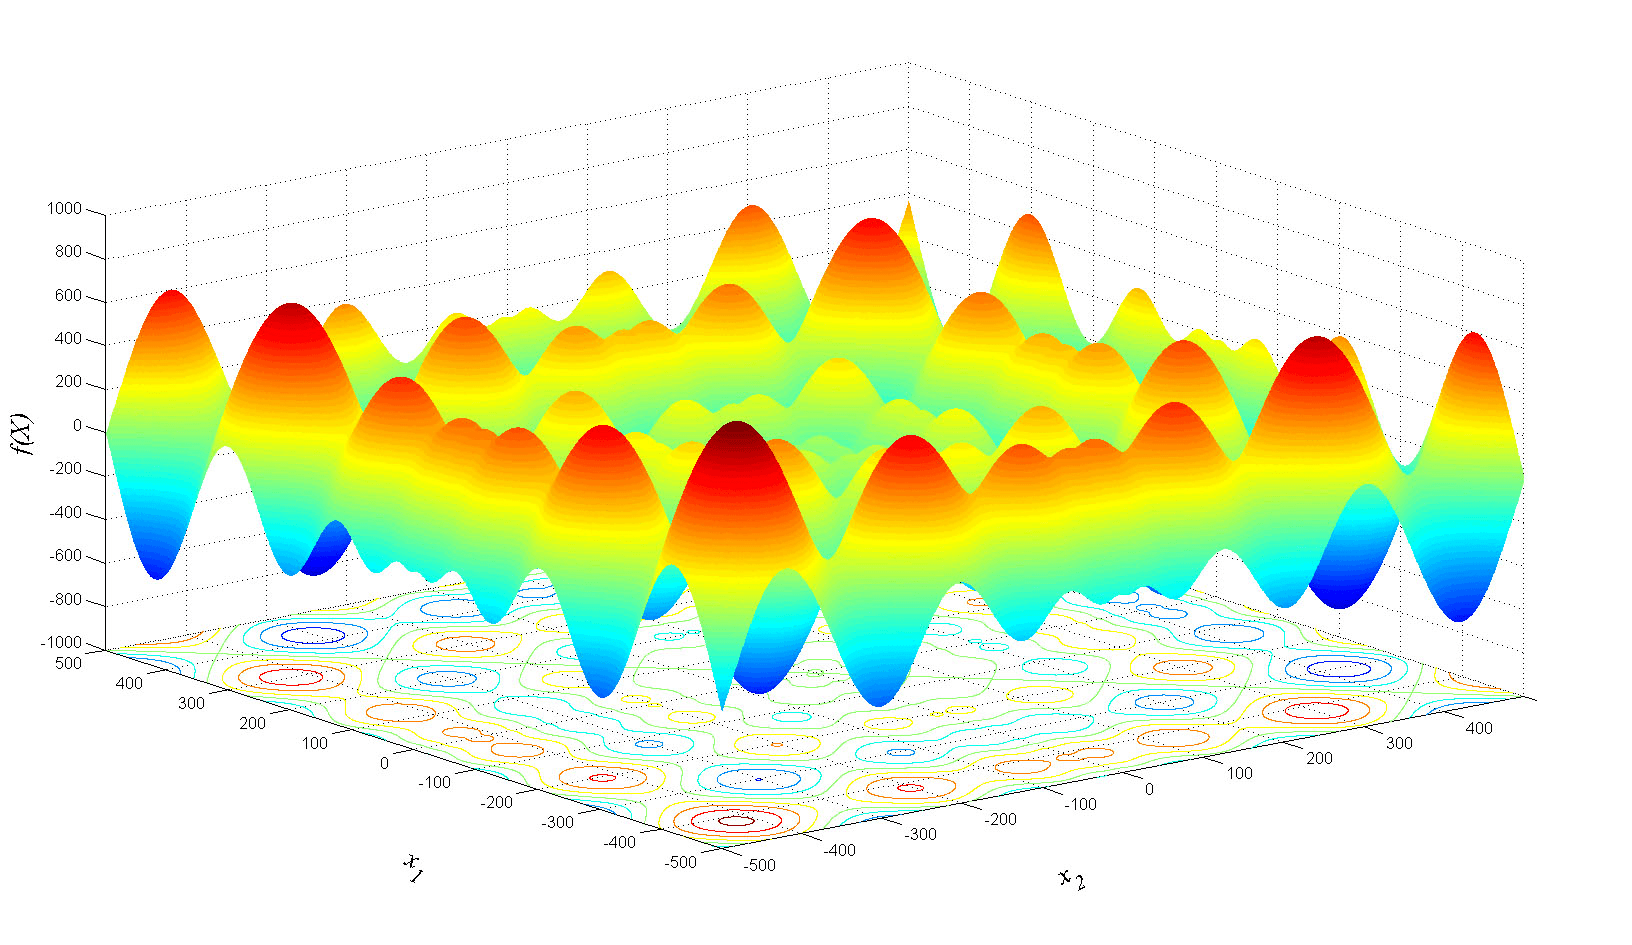
\includegraphics[width=100mm,scale=0.5]{Schwefel_fucntion}
  \caption{Image Schwefel's Function. \protect\footnotemark}
\end{figure}
\footnotetext{https://al-roomi.org/component/tags/tag/schwefel-function}

\begin{figure}[!h]
  \centering
  $$ f(x) = A \cdot n + \sum_{i=1}^n \left[ x_i^2 - A \cdot cos(2 \pi x_i) \right],
  A = 10, x_i \in \left[ -5.12, 5.15 \right]$$
   $$min = 0$$

  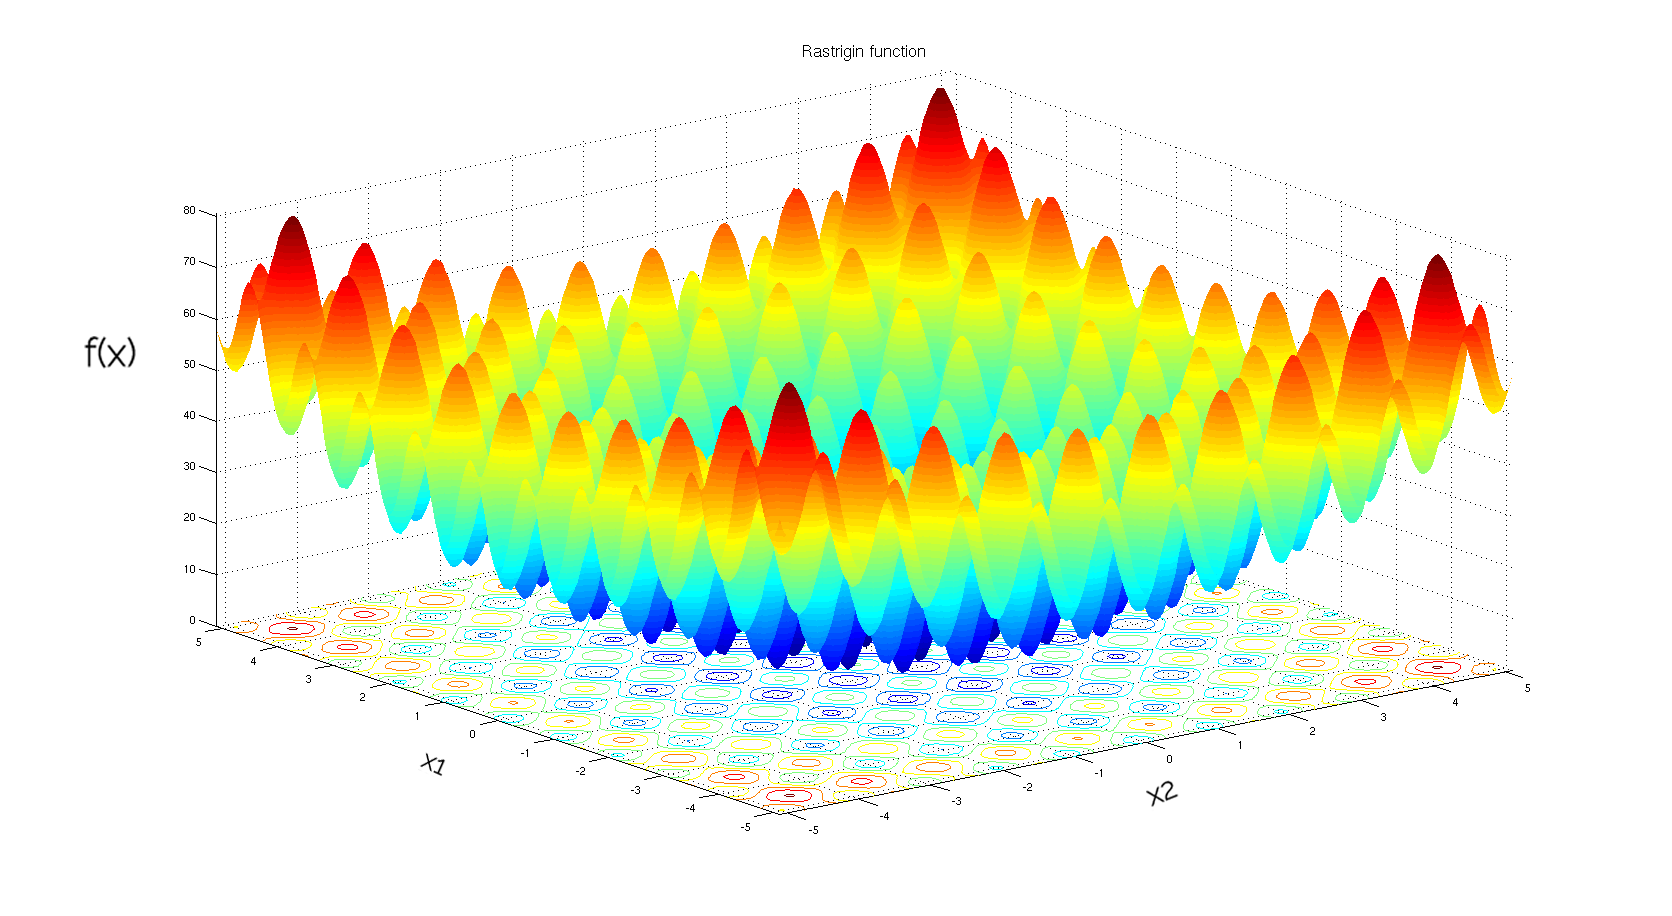
\includegraphics[width=100mm,scale=0.5]{Rastrigin_function}
  \caption{Image Rastrigin's Function. \protect\footnotemark}
\end{figure}
\footnotetext{https://commons.wikimedia.org/wiki/MainPage}

\pagebreak

\begin{figure}[!h]
  \centering
  $$ f(x) = -\sum_{i=1}^n \left[sin(x_i) \cdot \left( sin\left( \frac{i \cdot x_i^2}{\pi}  \right) \right)^{2 \cdot m} \right] ,
  x_i \in \left[ 0, \pi \right] ,  m = 10$$

   $$min = -4.68 \, , \, n = 5$$
   $$min = -9.66 \, , \, n = 10$$
   $$min < -27.5 \, , \, n = 30$$

  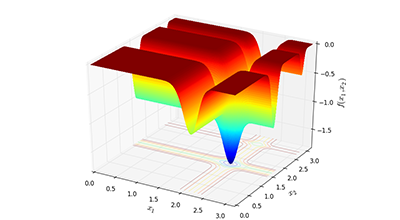
\includegraphics[width=100mm,scale=0.5]{Michalewicz_functions}
  \caption{Michalewicz's Function. \protect\footnotemark}
\end{figure}
\footnotetext{https://www.sfu.ca/~ssurjano/michal.html}

\pagebreak

\section*{Experiment}

The Hill Climbing and Simulate Anealing algorithms were implementen in python and analised the functions above with 100 iterations. The temperature for simulated aneealing is initialy 2000.
\newline
The Genetic algorithm was implemented in C++ and analised the functions above with a population of 1000, an elite population of 10 and 1000 iterations. The test was run on the compiled 64 bit program.
\newline
Each test has $10^{-5}$ precissionn is run 30 times to ensure consistancy.


\end{document}
